\documentclass[a4paper,12pt]{article}
%%%%%%%%%%%%%%%%%%%%%%%%%%%%%%%%%%%%%%%%%%%%%%%%%%%%%%%%%%%%%%%%%%%%%%%%%%%%%%%%%%%%%%%%%%%%%%%%%%%%%%%%%%%%%%%%%%%%%%%%%%%%%%%%%%%%%%%%%%%%%%%%%%%%%%%%%%%%%%%%%%%%%%%%%%%%%%%%%%%%%%%%%%%%%%%%%%%%%%%%%%%%%%%%%%%%%%%%%%%%%%%%%%%%%%%%%%%%%%%%%%%%%%%%%%%%
\usepackage{eurosym}
\usepackage{vmargin}
\usepackage{amsmath}
\usepackage{graphics}
\usepackage{epsfig}
\usepackage{subfigure}
\usepackage{framed}
\usepackage{enumerate}
\usepackage{fancyhdr}

\setcounter{MaxMatrixCols}{10}
%TCIDATA{OutputFilter=LATEX.DLL}
%TCIDATA{Version=5.00.0.2570}
%TCIDATA{<META NAME="SaveForMode"CONTENT="1">}
%TCIDATA{LastRevised=Wednesday, February 23, 201113:24:34}
%TCIDATA{<META NAME="GraphicsSave" CONTENT="32">}
%TCIDATA{Language=American English}

\pagestyle{fancy}
\setmarginsrb{20mm}{0mm}{20mm}{25mm}{12mm}{11mm}{0mm}{11mm}
\lhead{StatsResource} \rhead{Probability Distributions} \chead{ Uniform Distribution} %\input{tcilatex}

\begin{document}


\section*{Continuous Uniform Distribution: Subway Example}
Suppose there is a platform in a subway station in a large large city.  \\ Subway trains arrive \textbf{every three minutes} at this platform.
\begin{enumerate}[(a)]
\item   What is the shortest possible time a passenger would have to wait for a train?
\item What is the longest possible time a passenger will have to wait?
\item What is the probability that they will have to wait longer than 2 minutes?
\item What is the probability that they will have to wait less than than 45 seconds (i.e. 0.75 minutes)?
\item Compute the expected value and variance of the waiting time $X$.
\end{enumerate}


%------------------------------------------------------------------------%
{
\subsection*{Solution to Part A}

\begin{itemize}
\item What is the shortest possible time a passenger would have to wait for a train?
%\begin{itemize}
\item If the passenger arrives just before the doors close, then the waiting time is zero.
\[ a = 0 \mbox{ minutes } \]
\end{itemize}
\subsection*{Solution to Part B}
\begin{itemize}
\item What is the longest possible time a passenger will have to wait?
%\begin{itemize}
\item If the passenger arrives just after the doors close, and missing the train, then they will have to wait the full three minutes for the next one.
\[ b = 3 \mbox{ minutes }  = 180 \mbox{ seconds}  \]
\end{itemize}
%\end{itemize}
\subsection*{Solution to Part C}



\begin{itemize}
\item What is the probability that they will have to wait longer than 2 minutes?
\[ P(X \geq 2)  = {3-2 \over 3-0} = {1/3} = 0.3333   \]
\end{itemize}
%\end{itemize}


%% \vspace{-0.5cm}

\begin{center}
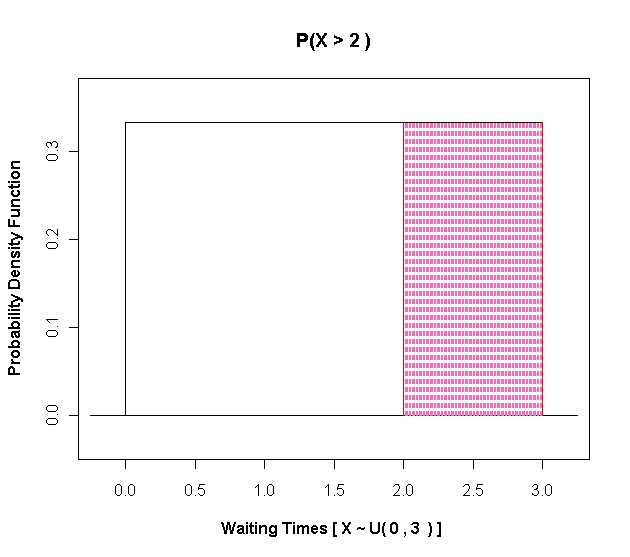
\includegraphics[scale=0.35]{images/6AUniform4}

\end{center}

\subsection*{Solution to Part D}

\begin{itemize}
\item What is the probability that they will have to wait less than than 45 seconds (i.e. 0.75 minutes)?
\[ P(X \leq 0.75)  = {0.75 - 0 \over 3-0} = {0.75/3} = 0.250  \]
\end{itemize}
%\end{itemize}

}




%% \vspace{-0.5cm}

\begin{center}
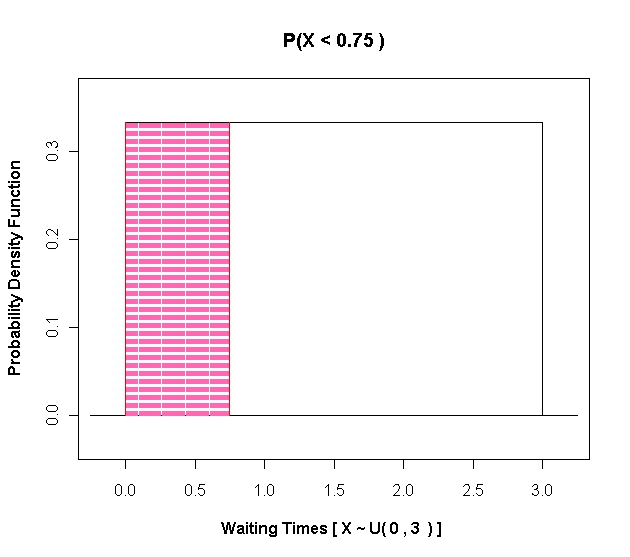
\includegraphics[scale=0.35]{images/6AUniform3}

\end{center}



\subsection*{Solution to Part E}

We are told that, for waiting times,  the lower limit $a$ is 0, and the upper limit $b$ is 3 minutes. \\ \bigskip The expected waiting time $\textrm{E}[X]$ is computed as follows
%% \vspace{0.1cm}
\[
\textrm{E}[X] = {b + a \over 2} =  {3 + 0  \over 2}  = 1.5 \mbox{ minutes }
\]


\noindent The variance of the continuous uniform distribution, denoted $\textrm{Var}(X)$,  is  computed using the following formula
%% \vspace{0.1cm}
\[
\textrm{Var}(X) = {(b - a)^2 \over 12} = {(3 - 0)^2 \over 12} =  {3^2 \over 12} = {9 \over 12} = 0.75
\]












\end{document}
